\newpage
\section{Setup and execution}
\label{sec:durchfuerung}
The first part of this section will describe the setup, the later the execution of the experiment.
\subsection{Setup}
A diagram of the setup is shown in figure \ref{fig:setup_scheme}, the actual experimental setup is shown in figure \ref{fig:setup_actual}.
\begin{figure}
    \begin{subfigure}{0.48\textwidth}%
        \centering
        \includegraphics[width=\textwidth]{content/pictures/aufbau_schema.png}
        \caption{Schematic of the expeimental setup. \cite{anleitung}}
        \label{fig:setup_scheme}
    \end{subfigure}%
    \hfill
    \begin{subfigure}{0.48\textwidth}%
        \centering
        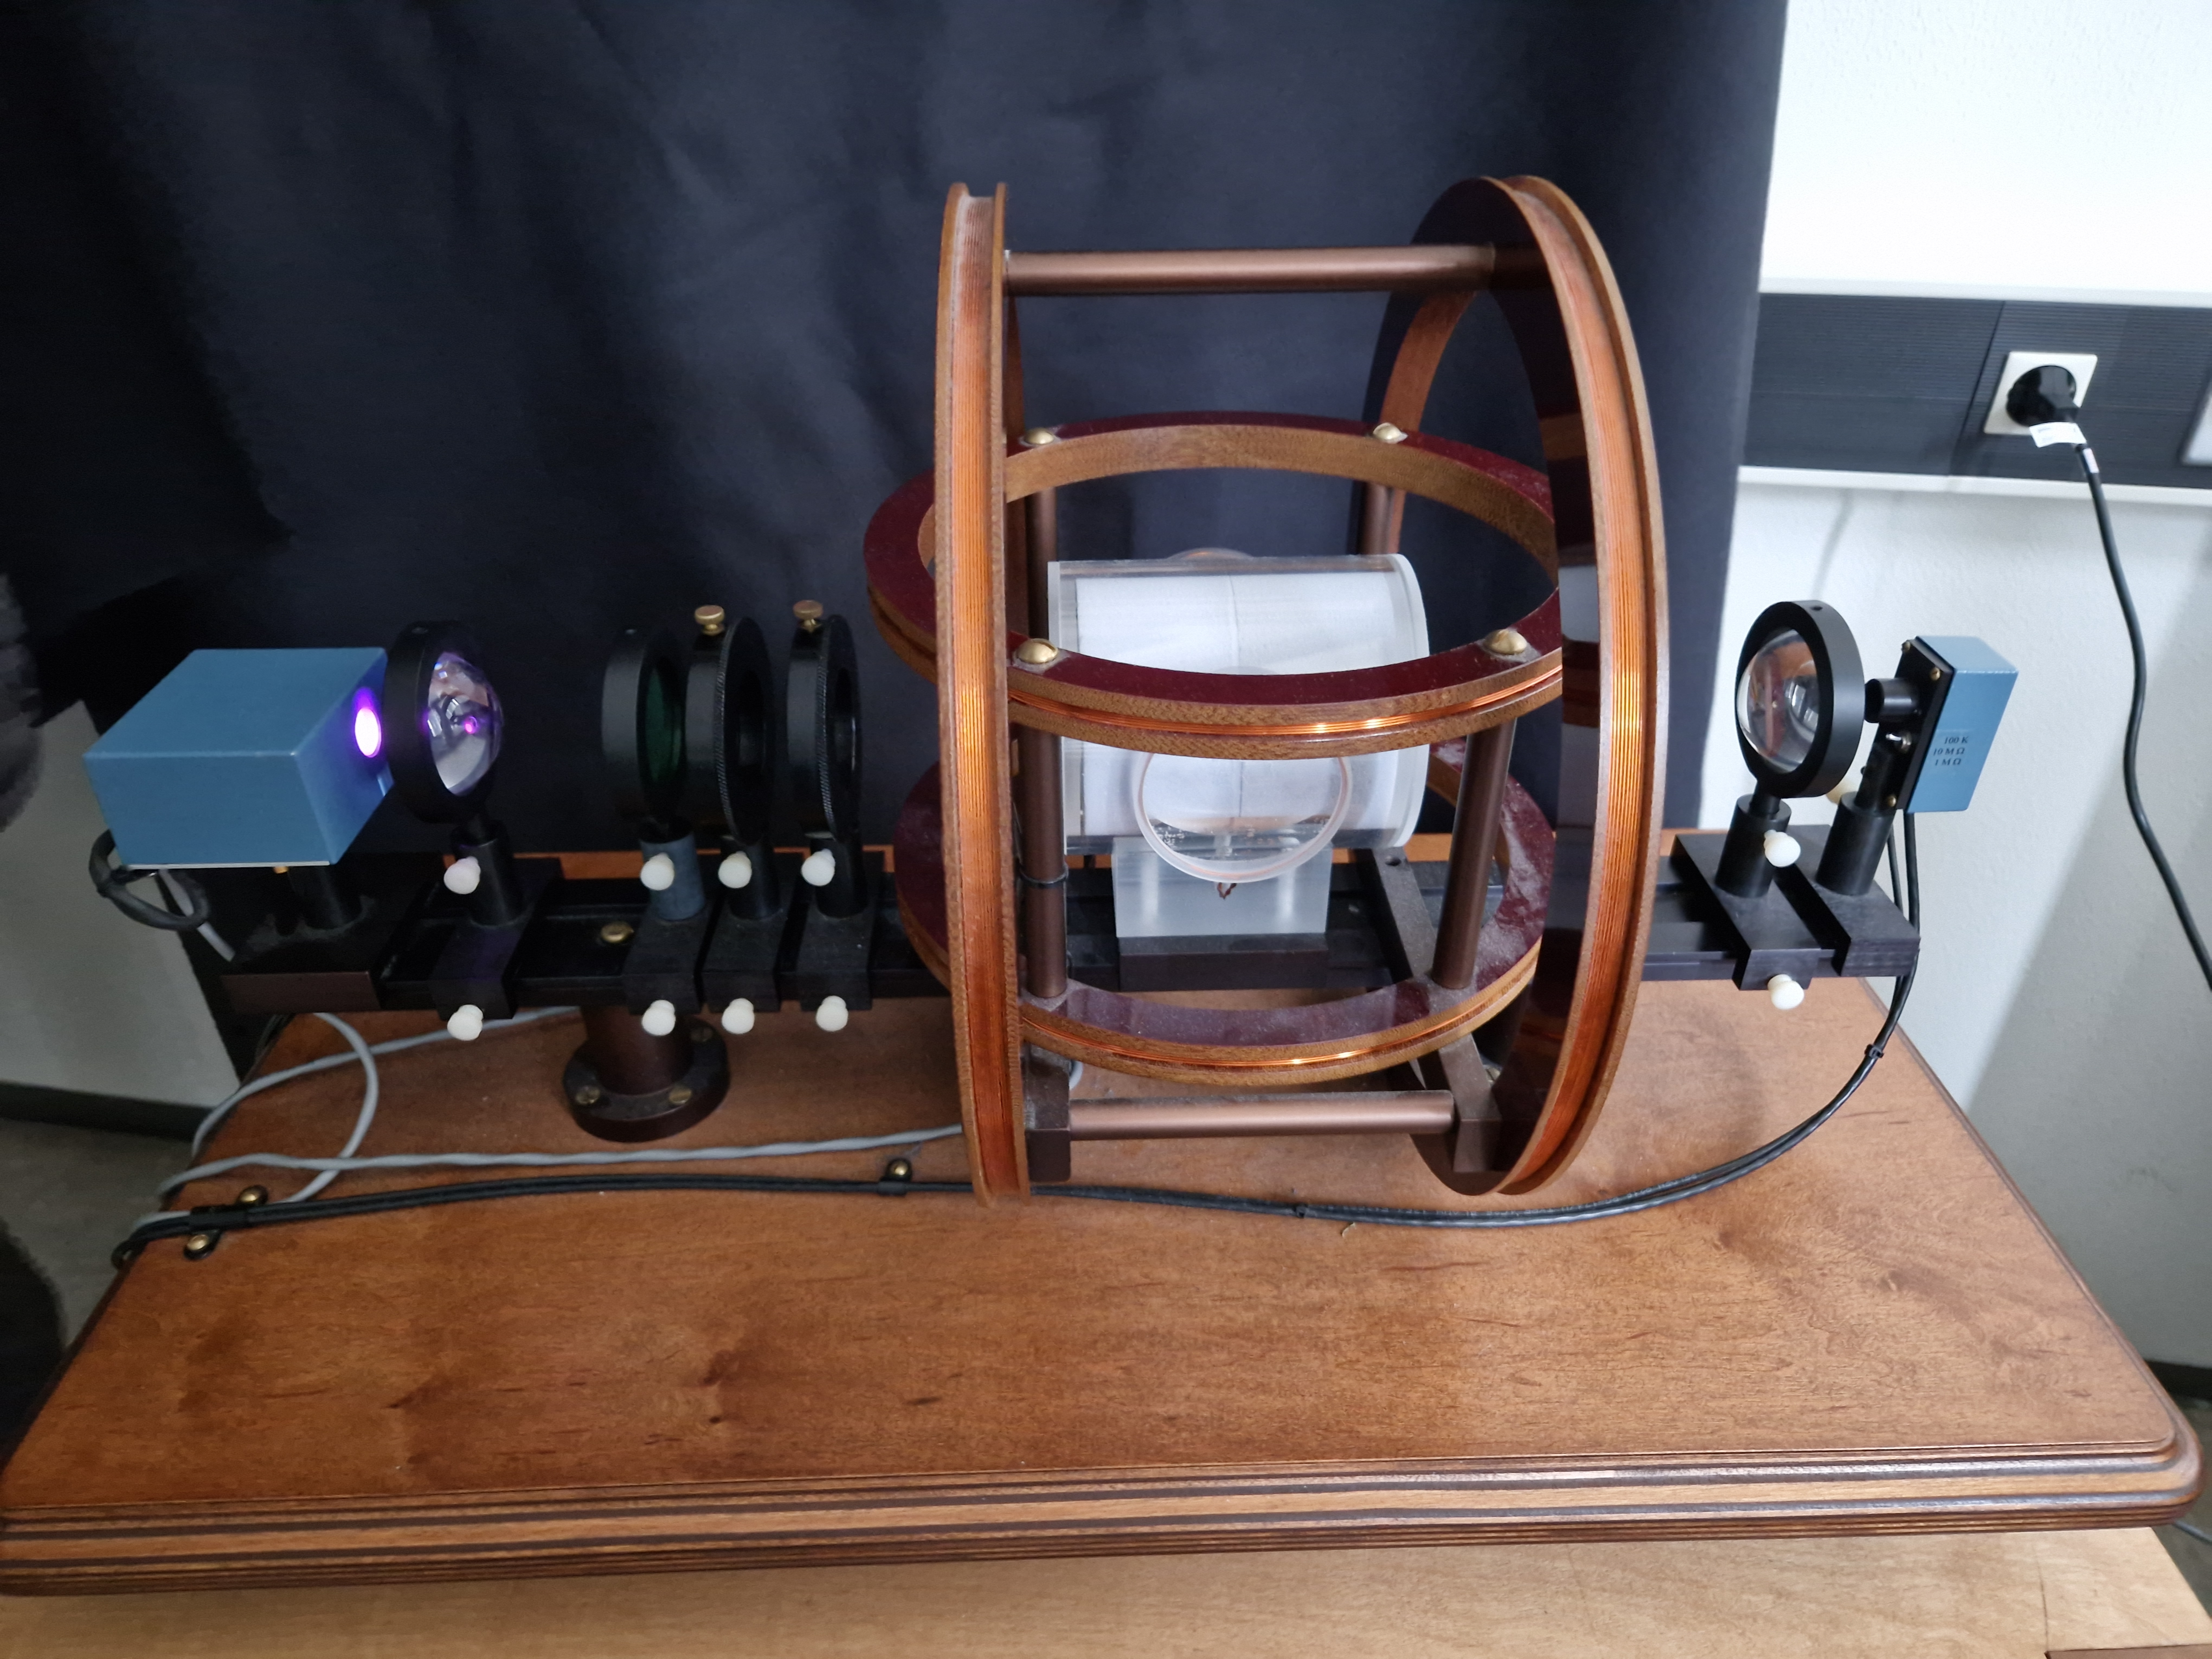
\includegraphics[width=\textwidth]{content/pictures/aufbau.jpeg}
        \caption{The actual experimental setup while the measuments are taken.}
        \label{fig:setup_actual}
    \end{subfigure}
    \caption{}
\end{figure}
As the main interest of this experiment is to measure the heat capacity at low temperatures two main things are needed
\begin{enumerate}
    \item Low temperatures
    \item Good heat isolation.
\end{enumerate}
To achieve the low temperatures, advatage is taken of a Dewar-vessel, which is filled with liquid nitrogen.
The Dewar-vessel contains a recipient in which the copper probe is contained.
Through the recipient the second thing that is needed can be achieved as a vacuum can be pumped inside the recipient.
Besides that the recipient is connected to a helium container and can be filled with helium.
This gives a high heat conduction to cool down the probe to liquid nitrogene temperatures.
On the other hand through the vacuum that is pumped afterwards a good heat isolation is achieved, the heat isolation is additionally aided by a heat shield which is located inside the recipient.\\
The probe is located inside the recipient and surrounded by the heat shield. 
Inside the heat shield and the probe are a wire to controle and measure the temperature of both.
The temperature of probe and heat shield is measured by a platinum 100 resistor.\\\\
As already mentioned the heat shield and the probe contain two separate wires.
Both of them have a voltage source to accurately apply a heating current.
Both voltage sources are connected to a volt-meter, so that the heat power that is put into the copper can later be determined.
A stop watch is used to monitor the time.

\subsection{Execution}
At first the copper probe needs to be cooled down.
To do so the Dewar-vessel is filled with liquid nitrogen and the recipient is flooded with helium.
The resistance of both the heat shield and the probe is constantly monitored, while waiting for the probe to cool down to liquid nitrogen temperatures.
After the probe and the heat shield reach the desired temperature, the helium bottle is disconnected from the recipient.
Moreover, a vacuum pump is connected to the recipient to pump a vacuum inside the probe chamber.
After some time the vacuum inside the recipient is sufficient to start the actual measurment. \\
Now the voltage source of the probe heater and the heat shield are turned on, the stop watch is turned on, the resistance of the platinum 100 at both the heat shield anmd the probe is written down aswell as the applied voltage and current at the probe heater.
Now every minute a new measument of heat shield and probe resistance is taken, the corresponding time and applied heat voltage and current is written down.
This process is repeated until the probe reaches room temperature levels.